\chapter{Transport Calculations with \wannier\ }\label{ch:transport}

By setting $\verb#transport#=\verb#TRUE#$, \wannier\ will calculate
the quantum conductance and density of states of a one-dimensional
system. The results will be written to files \verb#seedname_qc.dat#
and \verb#seedname_dos.dat#, respectively.

The system for which transport properties are calculated is determined
by the keyword \verb#transport_mode#.

\section{\tt transport\_mode = bulk}

Quantum conductance and density of states are calculated for a perfectly
periodic one-dimensional conductor. If $\verb#tran_read_ht#=\verb#FALSE#$
the transport properties are calculated using the Hamiltonian in the Wannier 
function basis of the system found by \wannier. Setting 
$\verb#tran_read_ht#=\verb#TRUE#$ allows the user to provide an 
external Hamiltonian matrix file {\tt seedname\_htB.dat}, from which
the properties are found. See Section~\ref{sec:post-p} for more details of 
the keywords required for such calculations.

\section{\tt transport\_mode = lcr}

Quantum conductance and density of states are calculated 
for a system where semi-infinite, left and right leads
are connected through a central conductor region. This is known 
as the \emph{lcr} system.
Details of the method is described in Ref. \cite{nardelli-prb99}.

In \wannier\ two options exist for performing such calculations: 
\begin{itemize}
\item If $\verb#tran_read_ht#=\verb#TRUE#$ the external Hamiltonian 
files {\tt seedname\_htL.dat, seedname\_htLC.dat, seedname\_htC.dat, 
seedname\_htCR.dat, seedname\_htR.dat} are read and used to compute 
the transport properties. 
\item If $\verb#tran_read_ht#=\verb#FALSE#$, then the transport
calculation is performed automatically using the Wannier functions as a
basis and the 2c2 geometry described in Section~\ref{sec:2c2}.
\end{itemize}

\section{Automated lcr Transport Calculations: The 2c2 Geometry}
\label{sec:2c2}

Calculations using the 2c2 geometry provide a method to calculate the
transport properties of an lcr system from a single \wannier\ calculation.
The Hamiltonian matrices which the five external files provide in the 
$\verb#tran_read_ht#=\verb#TRUE#$ case are instead built from the 
Wannier function basis directly. As such, strict rules apply to the system geometry, 
which is shown in Figure~\ref{fig:2c2}. These rules are as follows:
\begin{itemize}
\item Left and right leads must be identical and periodic.
\item Supercell must contain two principal layers (PLs) of lead on the left,
a central conductor region and two principal layers of lead on the right.
\item The conductor region must contain enough lead such that the
disorder does not affect the principal layers of lead either side.
\item A single \textbf{k}-point (Gamma) must be used.
\end{itemize}

\begin{figure}[h]
\centering
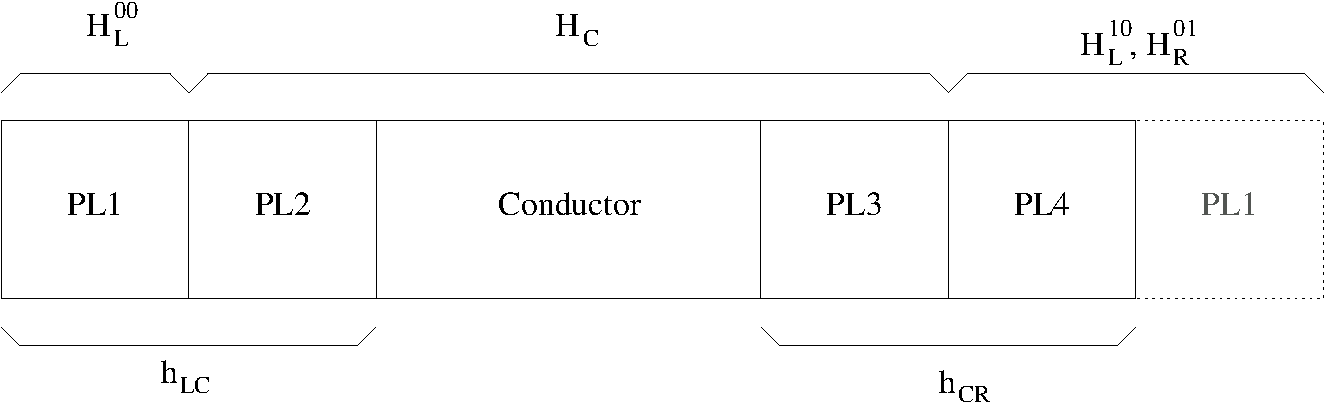
\includegraphics[height=4cm]{lcr_2c2}
\caption{Schematic illustration of the supercell required for 2c2
lcr calculations, showing where each of the Hamiltonian matrices
are derived from. Four principal layers (PLs) are required plus the
conductor region.}
\label{fig:2c2}
\end{figure}

In order to build the Hamiltonians, Wannier  functions are first 
sorted according to position and then type if a number of Wannier
functions exist with a similar centre (eg. \emph{d}-orbital type Wannier
functions centred on a Cu atom). Next, consistent parities of Wannier
function are enforced. To distingiush between different types of Wannier function
and assertain relative parities, a signature of each Wannier function 
is computed. The signature is formed of 20 integrals which have
different spatial dependence. They are given by:

\begin{equation}
I=\frac{1}{V}\int_V g(\mathbf{r})w(\mathbf{r})d\mathbf{r}
\label{eq:sig_ints}
\end{equation}

where $V$ is the volume of the cell, $w(\mathbf{r})$ is the Wannier 
function and $g(\mathbf{r})$ are the set of functions:

\begin{eqnarray}
g(\mathbf{r})=&\left\lbrace1,\sin\left(\frac{2\pi (x-x_c)}{L_x}\right),
											 \sin\left(\frac{2\pi (y-y_c)}{L_y}\right),
											 \sin\left(\frac{2\pi (z-z_c)}{L_z}\right),
											 \sin\left(\frac{2\pi (x-x_c)}{L_x}\right)
											 \sin\left(\frac{2\pi (y-y_c)}{L_y}\right),\right.\nonumber \\
										   &\left.\sin\left(\frac{2\pi (x-x_c)}{L_x}\right)
											 \sin\left(\frac{2\pi (z-z_c)}{L_z}\right),
											 ... \right\rbrace
\label{eq:g(r)}
\end{eqnarray}
upto third order in powers of sines. Here, the supercell has dimension 
$(L_x,L_y,L_z)$ and the Wannier function has centre $\mathbf{r}_c=(x_c,y_c,z_c)$.
Each of these integrals may be written as linear combinations 
of the following sums:

\begin{equation}
S_n(\mathbf{G})=\displaystyle{e^{i\mathbf{G.r}_{c}}\sum_{m}U_{mn}\tilde{u}_{m\Gamma}^{*}(\mathbf{G})}
\end{equation}

where $n$ and $m$ are the Wannier function and band indexes, 
$\mathbf{G}$ is a G-vector, $U_{mn}$ is the unitary matrix that 
transforms from the Bloch reopresentation of the system to the 
maximally-localised Wannier function basis and 
$\tilde{u}_{m\Gamma}^{*}(\mathbf{G})$ are the conjugates of the 
Fourier transforms of the periodic parts of the Bloch states at the $\Gamma\!$
-point. The complete set of $\tilde{u}_{m\mathbf{k}}(\mathbf{G})$ 
are often outputted by plane-wave DFT codes. However, to calculate the 20 
signature integrals, only 32 specific $\tilde{u}_{m\mathbf{k}}(\mathbf{G})$ 
are required. These are found in an additional file (\verb#seedname.unkg#) 
that should be provided by the interface between the DFT code and \wannier\ . 
A detailed description of this file may be found in Section~\ref{sec:files_unkg}.

Additionally, the following keywords are also required in the input file:
\begin{itemize}
\item \verb#tran_num_ll# : The number of Wannier functions in a 
principal layer.
\item \verb#tran_num_cell_ll# : The number of unit cells in one 
principal layer of lead
\end{itemize}

A further parameter related to these calculations is
\verb#tran_group_threshold#.

Examples of how 2c2 calculations are preformed can be found 
in the \wannier\ Tutorial. 
